\documentclass[10pt]{article}
\usepackage[preprint]{tmlr}
\usepackage{graphicx}
\usepackage{booktabs}
\usepackage{amsmath,amssymb}
\usepackage{url}
\usepackage{multirow}
\usepackage{array}
\usepackage{microtype}
\usepackage{enumitem}
\usepackage{hyperref}
\hypersetup{hidelinks}

\title{An Explainable and Imbalance-Aware Machine Learning Framework for Heart Disease Risk Prediction}

\author{
\name{Nirvaan Sinha}\\
\addr{ECE, BVCOEP}\\
\email{nsinga24-ece@bvucoep.edu.in}\\[0.15in]
\name{Sam Mendonca}\\
\addr{ECE, BVCOEP}\\
\email{smendonca24-ece@bvucoep.edu.in}
}

\begin{document}
\maketitle

\begin{abstract}
Machine learning has been increasingly investigated for clinical risk prediction, but predictive accuracy alone is insufficient when models are intended to support healthcare decisions. Two challenges are particularly important: class imbalance, which can cause classifiers to underperform on minority disease cases, and limited interpretability in complex models. This paper presents an explainable and imbalance-aware framework for heart disease risk prediction using the supplied \texttt{heart.csv}, a 13-predictor heart-disease dataset whose variables follow the commonly used Cleveland/UCI formulation. The framework compares logistic regression, decision trees, random forests, and a compact feed-forward neural network while investigating class-weighted learning and Synthetic Minority Over-sampling Technique (SMOTE). Model performance is evaluated using accuracy, precision, recall, F1-score, specificity, and ROC-AUC, with particular attention to minority-class recall. Interpretability is examined through decision-tree structure, feature importance, and SHAP-based feature attribution for complex models. The study is designed to quantify the trade-off between predictive performance and explainability rather than treating accuracy as the sole criterion. The resulting system is intended as a research and educational decision-support prototype and not as a substitute for professional medical diagnosis. The experiments are conducted on the supplied dataset after duplicate-record removal, with a fixed stratified 80/20 train/test split and random seed 42. \vspace{4pt}\textbf{KEYWORDS:} Heart disease, machine learning, binary classification, class imbalance, feature importance, SMOTE, logistic regression, decision tree, random forest, neural network, explainable AI, SHAP.\vspace{14pt}
\end{abstract}

\section{Introduction}
Heart disease remains an important application area for predictive machine learning because clinical datasets contain multiple interacting demographic, symptomatic, physiological, and diagnostic variables. Machine learning classifiers can learn associations between these variables and disease outcomes, potentially supporting risk stratification and decision-support workflows. However, a clinically oriented prediction system must be evaluated more carefully than a generic classification problem.

One issue is class imbalance. When one outcome is represented substantially more often than another, a classifier can obtain a high overall accuracy while performing poorly on the minority class. In a disease-prediction setting, this can be problematic because false-negative predictions correspond to disease cases that the classifier fails to identify. Consequently, evaluation should include metrics such as recall, precision, F1-score, specificity, and ROC-AUC rather than relying only on accuracy.

A second issue is interpretability. Logistic regression and shallow decision trees expose relatively understandable relationships between inputs and predictions, whereas ensemble models and neural networks can encode more complex decision functions. This creates a practical trade-off between predictive flexibility and the ability of a user to understand why a prediction was produced. Explainable artificial intelligence methods, including SHAP, provide a way to investigate feature contributions in otherwise complex models \citep{lundberg2017unified}.

This project develops a controlled comparison of interpretable and complex models on the UCI Heart Disease dataset. The central research questions are: (1) how does explicit treatment of class imbalance affect disease-prediction performance, and (2) how does predictive performance compare with model interpretability across traditional and neural models? The work emphasizes reproducibility, leakage prevention, and transparent reporting.

\section{Related Work}

\subsection{Machine Learning for Heart Disease Prediction}
Machine learning has been widely studied for cardiovascular risk prediction using structured clinical variables. Classical approaches such as logistic regression, decision trees, support vector machines, and random forests remain common because they can operate directly on tabular clinical measurements and provide useful baselines. Earlier studies on the Cleveland/UCI heart-disease data established the dataset as a benchmark for binary heart-disease classification, while later work has compared hybrid and ensemble approaches on related datasets \citep{alizadehsani2013data,haq2018hybrid,mohan2019effective,dwivedi2018performance}. More recent studies continue to evaluate multiple classifiers and feature-selection strategies, often combining public heart-disease datasets with additional cohorts \citep{alshaikh2024comprehensive,elsofany2024proposed,abdullah2024explainable}.

Deep learning has also become an active research direction. Reviews of heart-disease prediction literature report the use of feed-forward neural networks, convolutional architectures, recurrent approaches, and hybrid systems, while emphasizing the importance of dataset size, validation design, and interpretability \citep{zhou2024deep,alsekait2025cnn}. The present work uses a compact multilayer perceptron rather than a deep architecture because the deduplicated experimental dataset contains only 302 observations.

\subsection{Class Imbalance and Evaluation}
Class imbalance can distort accuracy and class-specific error rates. SMOTE creates synthetic minority observations by interpolating between minority-class examples \citep{chawla2002smote}, while class-weighted objectives change the relative training contribution of the classes. Recent heart-disease studies continue to use SMOTE alongside classifier comparisons and feature-selection procedures \citep{elsofany2024proposed,shah2025hybrid}. Because our supplied CSV contains a moderate rather than extreme class asymmetry after duplicate removal, imbalance handling is treated as an experimental variable rather than an assumption that the data are severely imbalanced.

For evaluation, accuracy is supplemented by precision, recall, F1-score, specificity, ROC-AUC, and PR-AUC. ROC analysis is a standard threshold-independent discrimination tool \citep{fawcett2006roc}, while precision-recall analysis is useful when positive-class performance deserves particular attention \citep{saito2015precision}.

\subsection{Explainable Machine Learning in Heartcare}
The use of explainable artificial intelligence has increased because predictive performance alone does not reveal why a model produces a particular output. SHAP provides additive feature attributions for individual predictions and global summaries \citep{lundberg2017unified}, while LIME provides local surrogate explanations for black-box models \citep{ribeiro2016should}. Recent heartcare surveys identify SHAP, LIME, feature importance, and related techniques as important tools for communicating model behavior \citep{sreeja2024explainability}. Recent empirical work has integrated SHAP with tree-based classifiers, SMOTE, and user-facing prediction systems \citep{elsofany2024proposed,ahmed2024ecg,ganie2025ensemble,cenitta2026xai}. Explainable ML has also been evaluated using richer clinical sources such as echocardiography, demonstrating that interpretable models can be compared with conventional risk scores and assessed on independent data \citep{molenaar2024echo}.

\subsection{Position of the Present Study}
The contribution of this study is deliberately narrower than the highly optimized systems reported in recent literature. Rather than introducing a new optimization algorithm, a large ensemble, or a new clinical dataset, the work performs a controlled comparison of logistic regression, a shallow decision tree, random forest, and a compact neural network on the supplied \texttt{heart.csv}. The study explicitly removes exact duplicate records before splitting, evaluates SMOTE within the training pipeline, compares an interpretable tree against a neural model, and reports both global and local-style interpretability artifacts. This design is intended to make the experimental choices transparent and reproducible on a small tabular dataset.

\section{Dataset}
The experimental source is the user-supplied file \texttt{heart.csv}. It contains 1,025 rows and 14 columns: 13 predictor variables and one binary target. Its feature names and target formulation match the commonly used Cleveland/UCI heart-disease representation, but the supplied file is not identical in size to the original UCI Cleveland database, which contains 303 instances; therefore, all reported experiments use the supplied CSV as the authoritative dataset rather than downloading or substituting another copy \citep{uciheart}. Inspection identified 723 duplicate rows. After removing exact duplicate records, 302 unique patient records remained, comprising 164 positive and 138 negative target observations. The 13 predictors are age, sex, chest-pain type, resting blood pressure, serum cholesterol, fasting blood sugar, resting electrocardiographic results, maximum heart rate achieved, exercise-induced angina, ST depression (oldpeak), ST-segment slope, number of major vessels, and thalassemia-related information. The variable definitions correspond to the commonly used Cleveland heart-disease formulation described by the UCI Machine Learning Repository \citep{uciheart}.

The predictive variables include age, sex, chest-pain type, resting blood pressure, serum cholesterol, fasting blood sugar indicator, resting electrocardiographic results, maximum heart rate achieved, exercise-induced angina, ST depression (oldpeak), ST-segment slope, number of major vessels, and thalassemia-related information. These variables mix demographic, symptom-related, physiological, and categorical clinical-test information, making the dataset suitable for comparing linear, tree-based, and nonlinear classifiers. The supplied CSV contains no missing values. Because the project uses the supplied CSV as the experimental source, preprocessing was performed on that file rather than substituting a different version of the dataset.

For binary classification, target value 0 is treated as absence of disease and target value 1 as presence of disease. The final deduplicated dataset contains 54.30\% positive and 45.70\% negative observations. Although the class distribution is not severely imbalanced, imbalance-handling experiments are retained to test whether class weighting or SMOTE changes minority-class behavior.

The 13 predictors span demographic, symptom-related, physiological, laboratory, and clinical-test variables. The supplied CSV contains no missing values. These variables are retained in their supplied numeric representation so that the experiment reproduces the provided dataset without introducing external preprocessing assumptions. The post-deduplication class distribution is 164 positive and 138 negative observations (54.30\% versus 45.70\%). Although the asymmetry is moderate rather than extreme, imbalance-handling experiments are retained to determine whether class weighting or SMOTE changes class-specific error behavior.

\section{Methodology}

\subsection{Data Preprocessing}
The preprocessing pipeline consists of duplicate inspection, missing-value inspection, train/test splitting, and model-specific scaling. Exact duplicate rows are removed before modeling, reducing the supplied data from 1,025 to 302 unique records. No missing values are present after this step. The data are divided into training and test sets using stratified sampling. Numerical features are standardized for logistic regression and the neural network; tree-based models are trained without scaling.

Let $X$ denote the input feature matrix and $y\in\{0,1\}$ denote the binary disease target. The deduplicated dataset is partitioned as
\begin{equation}
(X,y) = (X_{\mathrm{train}},y_{\mathrm{train}}) \cup (X_{\mathrm{test}},y_{\mathrm{test}}),
\end{equation}
where the two partitions are disjoint. Stratification is used so that both partitions retain approximately the same class proportions.


\subsection{Duplicate Detection and Leakage Prevention}
Duplicate handling is one of the most important preprocessing decisions in this project. The original CSV contains 1,025 rows, but 723 rows are exact duplicates, leaving 302 unique rows. If duplicated records were allowed to appear in both training and test partitions, a model could encounter a test row or an identical copy of it during training. Such overlap would make the test score optimistic because the model would be evaluated partly on repeated observations rather than independent examples.

The pipeline therefore removes exact duplicates before the train/test split. This decision is conservative: it reduces the amount of data available for learning, but it produces a cleaner separation between fitting and evaluation. The resulting 302-row dataset is split into 241 training observations and 61 test observations. The training set contains 131 positive and 110 negative examples; the test set contains 33 positive and 28 negative examples. These counts are used throughout the reported experiment.

No imputation is required because the supplied CSV contains no missing values. The preprocessing stage also does not use the target variable as an input feature. This separation prevents direct target leakage and makes the modeling task a standard supervised classification problem.

\subsection{Scaling and Pipeline Construction}
Feature scaling is used for logistic regression and the neural network because optimization can be affected when input variables have substantially different numeric ranges. Standardization transforms a feature $x_j$ according to
\begin{equation}
z_j=\frac{x_j-\mu_j}{\sigma_j},
\end{equation}
where $\mu_j$ and $\sigma_j$ are estimated from the training partition. The same transformation is then applied to the test partition without refitting the scaler.

Tree-based models do not require standardization because their splitting rules depend on ordered thresholds rather than distances or gradient magnitudes across feature dimensions. Keeping the tree models unscaled also makes their rule structure easier to interpret.

For the SMOTE configurations, oversampling is embedded in the training pipeline. This ordering is important: the test set remains untouched, and synthetic observations are generated only from training examples. The pipeline design is therefore part of the experimental methodology rather than a cosmetic implementation detail.

\subsection{Class-Imbalance Treatment}
Three training configurations are considered. The first uses the original training distribution without explicit imbalance correction. The second uses class-weighted learning, where errors from the minority class receive increased weight. The third uses SMOTE on the training partition only.

For a binary classifier, a weighted cross-entropy objective can be represented as
\begin{equation}
\mathcal{L} = -\sum_{i=1}^{N} w_{y_i}\left[y_i\log(\hat{p}_i)+(1-y_i)\log(1-\hat{p}_i)\right],
\end{equation}
where $w_{y_i}$ is the weight associated with the true class and $\hat{p}_i$ is the predicted probability for observation $i$.

SMOTE creates synthetic observations from minority-class neighborhoods. Crucially, it is applied after the train/test split and never to the held-out test set. This prevents synthetic examples derived from test observations from influencing training and avoids a direct form of data leakage.

\subsection{Logistic Regression}
Logistic regression is used as a transparent baseline. For an input vector $x$, the probability of disease is
\begin{equation}
P(y=1\mid x) = \sigma(\beta_0 + \beta^T x),
\end{equation}
where $\sigma(z)=1/(1+e^{-z})$ is the logistic sigmoid function. The fitted coefficients provide an interpretable description of the direction and magnitude of the model's linear associations, subject to the usual limitations of observational prediction.

\subsection{Decision Tree}
A decision tree recursively partitions the feature space using threshold-based rules. A constrained maximum depth is used to reduce overfitting and maintain a structure that can be inspected directly. The resulting tree can be visualized as a sequence of decisions from the root to a terminal node, making it the principal intrinsically interpretable model in this study.

\subsection{Random Forest}
Random forest combines predictions from multiple decision trees. For $M$ trees, a simplified binary classification rule is
\begin{equation}
\hat{y} = \operatorname{mode}\{T_1(x),T_2(x),\ldots,T_M(x)\}.
\end{equation}
The ensemble is included to determine whether combining trees improves predictive performance relative to a single interpretable tree while retaining some post-hoc feature-importance information.

\subsection{Neural Network}
The complex model is a feed-forward neural network with a small architecture appropriate for tabular data. The implemented network contains 13 standardized inputs, a first hidden layer with 64 units, a second hidden layer with 32 units, ReLU activations, and a single output unit. The output is converted to a class probability through the logistic sigmoid function. Adam optimization is used with an initial learning rate of $10^{-3}$ and L2 regularization through the MLP regularization parameter.

Early stopping is enabled using a validation fraction taken from the training data. Training stops when the validation objective fails to improve for the configured patience period. This is preferable to simply increasing the number of epochs on a small dataset, where the model could otherwise memorize idiosyncrasies of the training sample. The network is intentionally compact because the effective dataset contains only 302 unique observations.

\section{Experimental Protocol}
All models are trained using the same training/test partition and evaluated on the same untouched test data. After deduplication, the stratified split contains 241 training observations and 61 test observations; the training partition contains 131 positive and 110 negative cases, while the test partition contains 33 positive and 28 negative cases. The project uses fixed, explicitly documented hyperparameters rather than a large automated hyperparameter search. This keeps the experiment reproducible and avoids presenting repeated test-set experimentation as model tuning.

The principal experimental comparisons are: (1) models without explicit imbalance correction versus class-weighted models, (2) models trained after SMOTE versus their non-SMOTE counterparts, and (3) interpretable models versus more complex ensemble and neural models.

The experiment uses an 80/20 stratified train/test split with random seed 42. Logistic regression uses a maximum of 2,000 iterations. The decision tree uses maximum depth 4 and balanced class weights. The random forest uses 300 trees and balanced class weights. The neural network uses two hidden layers with 64 and 32 units, ReLU activation, Adam optimization, L2 regularization, early stopping, and a maximum of 1,000 training iterations. SMOTE and standardization are applied within the training pipeline before fitting the network. SMOTE uses random seed 42 and is applied only to the training partition.

\section{Evaluation Metrics}
Because disease prediction is potentially sensitive to class imbalance, multiple metrics are reported.

Accuracy is defined as
\begin{equation}
\mathrm{Accuracy}=\frac{TP+TN}{TP+TN+FP+FN}.
\end{equation}

Precision is
\begin{equation}
\mathrm{Precision}=\frac{TP}{TP+FP},
\end{equation}
while recall (sensitivity) is
\begin{equation}
\mathrm{Recall}=\frac{TP}{TP+FN}.
\end{equation}

The F1-score is the harmonic mean of precision and recall:
\begin{equation}
F_1=2\frac{\mathrm{Precision}\times\mathrm{Recall}}{\mathrm{Precision}+\mathrm{Recall}}.
\end{equation}

Specificity is calculated as
\begin{equation}
\mathrm{Specificity}=\frac{TN}{TN+FP}.
\end{equation}

ROC-AUC is used as a threshold-independent discrimination measure. Because ROC-AUC can sometimes obscure performance on rare positive classes, precision-recall curves are also considered when interpreting the imbalance experiments.


For the present dataset, the confusion matrix is also important because it exposes the practical error types hidden by aggregate scores. True positives are correctly identified positive cases, false negatives are positive cases classified as negative, true negatives are correctly identified negative cases, and false positives are negative cases classified as positive. In a research prototype, these counts are descriptive rather than clinical risk estimates.

The precision-recall area under the curve (PR-AUC) is additionally retained in the project reports because it focuses more directly on the precision-recall trade-off. In the executed experiment, PR-AUC values were 0.895 for logistic regression, 0.897 for balanced logistic regression, 0.901 for logistic regression with SMOTE, 0.820 for the decision tree, 0.899 for the random forest, and 0.912 for the neural network. These values complement ROC-AUC rather than replacing it.

\section{Explainability Analysis}

\subsection{Intrinsic Interpretability}
The decision tree is interpreted directly through its learned branching structure. The tree visualization exposes the sequence of feature-based conditions leading to each terminal classification. Feature importance measures are additionally reported for tree-based models.

\subsection{SHAP-Based Explanations}
For complex models, SHAP values are used to quantify feature contributions. The additive explanation can be expressed as
\begin{equation}
f(x)=\phi_0+\sum_{j=1}^{p}\phi_j,
\end{equation}
where $\phi_0$ is the expected model output and $\phi_j$ represents the contribution of feature $j$ for a particular observation \citep{lundberg2017unified}.

Global SHAP summaries can identify features that have the greatest influence across the dataset, while local explanations can show which features contributed toward or away from a particular prediction. These explanations describe model behavior and should not be interpreted as evidence of causal relationships.

\section{Results}
The results below were generated from the supplied CSV after duplicate removal. All models were evaluated on the same untouched 20\% test partition containing 61 observations.

\begin{table}[t]
\caption{Model performance comparison on the held-out test set. Values are rounded to three decimal places.}
\label{tab:results}
\centering
\begin{tabular}{lcccccc}
\toprule
Model & Accuracy & Precision & Recall & F1 & Specificity & ROC-AUC\\
\midrule
Majority baseline & 0.541 & 0.541 & 1.000 & 0.702 & 0.000 & 0.500\\
Logistic regression & 0.803 & 0.800 & 0.848 & 0.824 & 0.750 & 0.871\\
Logistic + class weights & 0.787 & 0.794 & 0.818 & 0.806 & 0.750 & 0.873\\
Logistic + SMOTE & 0.820 & 0.844 & 0.818 & 0.831 & 0.821 & 0.881\\
Decision tree & 0.721 & 0.750 & 0.727 & 0.738 & 0.714 & 0.833\\
Random forest & 0.770 & 0.788 & 0.788 & 0.788 & 0.750 & 0.874\\
Neural network & 0.820 & 0.844 & 0.818 & 0.831 & 0.821 & 0.886\\
\bottomrule
\end{tabular}
\end{table}

The majority-class baseline achieved 0.541 accuracy and 1.000 recall but zero specificity, demonstrating why accuracy alone is inadequate. Logistic regression achieved 0.803 accuracy and 0.871 ROC-AUC. Class weighting slightly reduced accuracy to 0.787 while maintaining 0.750 specificity. SMOTE produced the strongest overall result among the tested configurations, with 0.820 accuracy, 0.831 F1-score, 0.821 specificity, and 0.881 ROC-AUC. The decision tree achieved 0.721 accuracy and 0.833 ROC-AUC, while the random forest achieved 0.770 accuracy and 0.874 ROC-AUC. The neural network achieved 0.820 accuracy, 0.831 F1-score, and 0.886 ROC-AUC. Its ROC-AUC was the highest among the tested configurations, although its accuracy and F1-score were equal to those of logistic regression with SMOTE to the reported precision. Because the study uses a single held-out split, these small differences should not be interpreted as evidence of a definitive model ranking.


Figure~\ref{fig:performance} visualizes accuracy and ROC-AUC together. The closeness of several scores is important: differences of only a few percentage points on a 61-observation test set correspond to only a small number of cases. For this reason, the numerical results should be read together with the confusion matrices and the study limitations.

\begin{figure}[t]
\centering
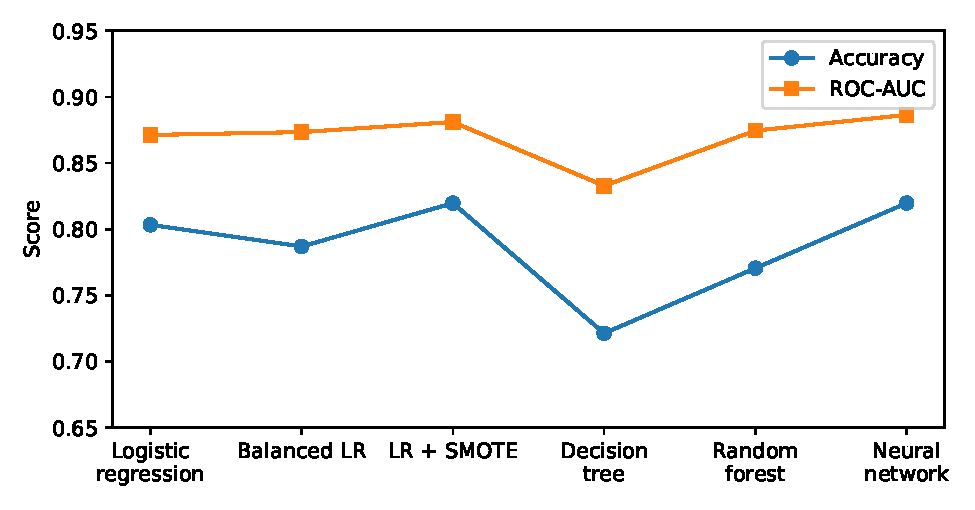
\includegraphics[width=0.88\linewidth]{figures/performance.pdf}
\caption{Accuracy and ROC-AUC for the six trained predictive configurations.}
\label{fig:performance}
\end{figure}

\begin{table}[t]
\caption{Confusion-matrix counts for the held-out test set.}
\label{tab:confusion}
\centering
\small
\begin{tabular}{lrrrr}
\toprule
Model & TN & FP & FN & TP\\
\midrule
Logistic regression & 21 & 7 & 5 & 28\\
Logistic + class weights & 21 & 7 & 6 & 27\\
Logistic + SMOTE & 23 & 5 & 6 & 27\\
Decision tree & 20 & 8 & 9 & 24\\
Random forest & 21 & 7 & 7 & 26\\
Neural network & 23 & 5 & 6 & 27\\
\bottomrule
\end{tabular}
\end{table}

The confusion matrices show why the SMOTE logistic model and the neural network have similar aggregate accuracy: both produce 23 true negatives, 5 false positives, 6 false negatives, and 27 true positives on the test set. Their ROC-AUC values differ because ROC-AUC uses the ranking of predicted scores across thresholds rather than only the single classification threshold used for the confusion matrix. Thus, two models can make the same thresholded decisions while producing different probability rankings.

\subsection{Illustrative Model Outputs}
To make the experimental results concrete, Table~\ref{tab:samples} shows three illustrative observations taken from the same 61-observation held-out test partition used for the aggregate evaluation. The examples are presented only to demonstrate model behavior; they are not clinical case studies and the numerical probabilities should not be interpreted as calibrated patient risk estimates. The neural network probability is the predicted probability of target class 1 from the fitted MLP pipeline, while the decision-tree and random-forest values are their corresponding class-1 probabilities.

\begin{table}[t]
\caption{Illustrative held-out test-set predictions from the trained models.}
\label{tab:samples}
\centering
\small
\begin{tabular}{rrrrrrrrrr}
\toprule
Age & Sex & CP & MaxHR & CA & Thal & Actual & DT & NN & RF \\
\midrule
41 & 1 & 2 & 168 & 0 & 2 & 1 & 1.000 & 0.814 & 0.860 \\
61 & 0 & 0 & 146 & 0 & 3 & 0 & 0.000 & 0.146 & 0.113 \\
67 & 1 & 2 & 150 & 0 & 3 & 0 & 0.577 & 0.481 & 0.773 \\
\bottomrule
\end{tabular}
\end{table}

For the first observation, the decision tree, neural network, logistic regression with SMOTE, and random forest all predicted class 1, with neural-network probability 0.814 and random-forest probability 0.860; the held-out target was 1. For the second observation, all four models predicted class 0, with neural-network probability 0.146 and random-forest probability 0.113; the held-out target was 0. The third observation illustrates model disagreement: the decision tree and random forest predicted class 1, whereas the neural network and SMOTE logistic model predicted class 0. The actual held-out target was 0. This example illustrates why model comparison should include both thresholded predictions and probability-based discrimination measures.

\subsection{Interpretability Results}
The decision tree provides direct rule-based interpretability, while the random forest provides aggregate feature-importance estimates. In the fitted random forest, the largest impurity-based importance values were associated with chest-pain type (cp, 0.163), maximum heart rate (thalach, 0.124), number of major vessels (ca, 0.113), thalassemia-related information (thal, 0.098), and ST depression (oldpeak, 0.091). SHAP analysis of the held-out predictions produced a similar global ordering, with cp, ca, thal, exercise-induced angina (exang), and thalach among the largest mean absolute attributions. These explanations describe model behavior rather than clinical causation.

The interpretation should avoid unsupported clinical claims. For example, a feature receiving a large SHAP value means that the feature strongly influenced the model output for the analyzed observation; it does not establish that the feature caused the disease.


Table~\ref{tab:rfimportance} reports the leading impurity-based feature-importance values from the fitted random forest. The corresponding figure makes the relative scale easier to inspect. The decision tree also assigned its largest importance to $cp$ (0.469), followed by $ca$ (0.153), $thal$ (0.112), $oldpeak$ (0.065), and $exang$ (0.061). These values are useful for describing the learned model, but they should not be interpreted as estimates of biological importance.

\begin{table}[t]
\caption{Leading random-forest feature importances.}
\label{tab:rfimportance}
\centering
\small
\begin{tabular}{lr}
\toprule
Feature & Importance\\
\midrule
cp & 0.163\\
thalach & 0.124\\
ca & 0.113\\
thal & 0.098\\
oldpeak & 0.091\\
age & 0.083\\
chol & 0.076\\
exang & 0.074\\
trestbps & 0.068\\
sex & 0.039\\
\bottomrule
\end{tabular}
\end{table}

\begin{figure}[t]
\centering
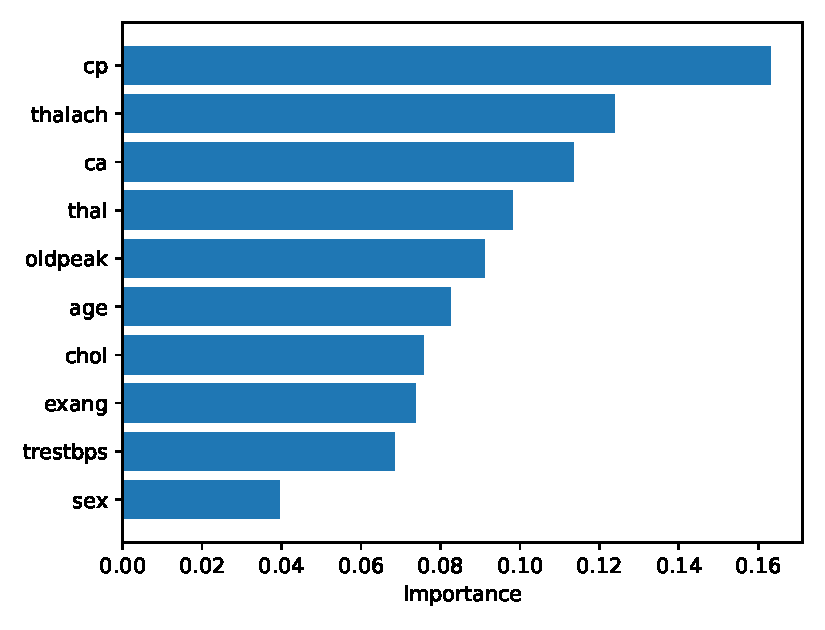
\includegraphics[width=0.78\linewidth]{figures/rf_importance.pdf}
\caption{Leading impurity-based feature importances from the fitted random forest.}
\label{fig:rfimportance}
\end{figure}

The neural network is less directly interpretable than the decision tree, so permutation importance was also computed. The largest mean ROC-AUC decreases under permutation were associated with $thal$ (0.036), $sex$ (0.035), $ca$ (0.033), $oldpeak$ (0.028), and $thalach$ (0.023). The fact that the neural network's permutation ranking is not identical to the random forest ranking is not unexpected: different models can rely on different combinations of correlated or interacting variables.

SHAP was applied to the random forest to provide additive feature-attribution explanations. At the global level, SHAP summarizes the magnitude of contributions across observations; at the local level, it can explain why a particular model output moved above or below the model's baseline expectation. The explanation therefore concerns the fitted predictor, not the underlying disease mechanism. In particular, a high attribution for a variable does not establish that changing that variable would cause the disease risk to change in the same direction.

\section{Discussion}
The central purpose of this study is to examine predictive performance together with interpretability. Recent literature similarly emphasizes that high predictive scores should be considered alongside validation design and explainability, particularly when models are intended for healthcare settings \citep{alshaikh2024comprehensive,sreeja2024explainability,ganie2025ensemble,cenitta2026xai}. The majority baseline illustrates the weakness of accuracy alone: it obtained 0.541 accuracy and 1.000 recall by predicting the positive class for every test observation, but specificity was 0.000. Among the trained models, logistic regression with SMOTE obtained the highest accuracy (0.820), F1-score (0.831), specificity (0.821), and ROC-AUC (0.881) on the held-out test set. Class weighting did not improve the selected metrics relative to the unweighted logistic model, while the decision tree provided direct interpretability at the cost of lower predictive performance on this split.

The final comparison distinguishes discrimination, class-specific error behavior, and explainability. The random forest produced ROC-AUC close to the logistic models but lower accuracy than logistic regression with SMOTE. The neural network also did not exceed the simpler models on the reported metrics. The decision tree was the most directly inspectable model because each prediction can be traced through explicit feature thresholds. These results illustrate that model complexity does not automatically translate into better performance on a small tabular dataset.

The neural network was included to test whether increased model complexity produces meaningful gains on the small tabular dataset. Its ROC-AUC of 0.886 was the highest reported value in the experiment, while its accuracy and F1-score matched the logistic-regression-with-SMOTE configuration at the reported precision. This result supports a more nuanced interpretation: the neural network learned useful nonlinear decision structure, but the observed advantage is modest and is not sufficient, on a single small test split, to establish superiority or clinical usefulness.

\section{Reproducibility and Software Organization}
The project separates data loading, training, evaluation, explanation, and application code. The training script loads the supplied CSV, removes exact duplicates, creates the stratified split, fits the documented configurations, computes metrics, and saves model artifacts. A fixed random seed of 42 is used for stochastic components, improving reproducibility across reruns. A complete rerun installs the dependencies in \texttt{requirements.txt} and executes \texttt{python run\_project.py}; the Streamlit application then loads the saved artifacts rather than retraining them.

\section{Limitations}
This study has several limitations. First, the effective dataset is small: duplicate removal reduces 1,025 supplied rows to 302 unique observations, and only 61 observations are reserved for the final test set. Consequently, the reported percentages can change materially with a different split. A stronger future evaluation should use repeated stratified cross-validation inside the training process and a genuinely independent external test cohort.

Second, the dataset is historical and may not represent current clinical populations, equipment, referral patterns, or healthcare settings. Even a model that performs well on the supplied file could experience distribution shift when deployed elsewhere. Third, synthetic oversampling changes the training distribution and does not create new real patient observations. SMOTE is therefore a modeling technique, not a substitute for collecting representative data.

Fourth, the study does not include probability calibration analysis, decision-curve analysis, prospective validation, subgroup fairness analysis, or external clinical validation. These omissions matter because discrimination metrics alone do not establish whether predicted probabilities are reliable or whether the system improves clinical outcomes.

Fifth, model explanations are explanations of learned associations rather than causal evidence. Feature importance can also be affected by correlated predictors, model structure, and the chosen explanation method. Finally, performance on a public benchmark does not establish clinical validity or safety. The system should therefore be considered a research and educational prototype and must not be used as an autonomous diagnostic tool or as a substitute for evaluation by a qualified healthcare professional.


\section{Broader Impact}
A transparent disease-risk model could potentially support educational demonstrations of how machine learning can assist clinical decision-making. However, incorrect predictions can cause harm if they are interpreted as medical diagnoses. Particular care is therefore required around false negatives, calibration, population shift, and demographic bias.

The framework deliberately reports multiple metrics and explanations rather than presenting a single accuracy value as proof of clinical usefulness. A model can be accurate on a benchmark yet poorly calibrated, unstable across populations, or inappropriate for a particular decision threshold. Any real deployment would require independent clinical validation, appropriate governance, privacy protections, monitoring, calibration assessment, and evaluation across relevant patient populations.

There is also a communication risk. Visual interfaces can make a probability look more authoritative than it is. The prototype should therefore present model output as an algorithmic estimate generated from a historical dataset. It should not imply certainty, diagnosis, or recommended treatment. In an educational setting, this limitation is part of the project's intended lesson: responsible machine learning requires attention to data quality, evaluation design, and explanation in addition to model accuracy.

\section{Conclusion}
This paper presents an explainable and imbalance-aware framework for heart disease risk prediction, comparing linear, tree-based, ensemble, and neural models under explicit imbalance-handling and explainability procedures. SMOTE improved the tested logistic-regression configuration on several metrics, while the neural network produced the highest ROC-AUC. The decision tree offered the most direct rule-based explanation, and the random forest supplied nonlinear capacity with post-hoc feature attribution.

The results support a methodological conclusion rather than a clinical ranking: model complexity should be justified empirically. Because the effective dataset is small and evaluation uses one held-out split, the observed differences are uncertain. Future work should prioritize repeated cross-validation, external validation, probability calibration, subgroup analysis, threshold analysis, and prospective evaluation. Until such validation is performed, the system remains a research and educational artifact rather than a clinical diagnostic tool.

\section*{Acknowledgments}
The authors acknowledge the UCI Machine Learning Repository for providing the Heart Disease dataset used in this study.

{\small\setlength{\itemsep}{0pt}
\begin{thebibliography}{99}

\bibitem[Mesquita and Marques(2024)]{abdullah2024explainable}
F. Mesquita and G. Marques.
\newblock An explainable machine learning approach for automated medical decision support of heart disease.
\newblock \emph{Data \& Knowledge Engineering}, 153:102339, 2024. doi:10.1016/j.datak.2024.102339.

\bibitem[Majhi and Kashyap(2024)]{ahmed2024ecg}
B. Majhi and A. Kashyap.
\newblock Explainable AI-driven machine learning for heart disease detection using ECG signal.
\newblock \emph{Applied Soft Computing}, 167:112225, 2024. doi:10.1016/j.asoc.2024.112225.

\bibitem[Al-Alshaikh et~al.(2024)]{alshaikh2024comprehensive}
H. A. Al-Alshaikh, P. P, R. C. Poonia, A. K. J. Saudagar, M. Yadav, H. S. AlSagri, and A. A. AlSanad.
\newblock Comprehensive evaluation and performance analysis of machine learning in heart disease prediction.
\newblock \emph{Scientific Reports}, 14:7819, 2024. doi:10.1038/s41598-024-58489-7.

\bibitem[Alizadehsani et~al.(2013)]{alizadehsani2013data}
R. Alizadehsani, J. Habibi, M. Hosseini, H. Mashayekhi, R. Bogdan, A. Ghandeharioun, B. Bahadorian, and Z. Sani.
\newblock A data mining approach for diagnosis of coronary artery disease.
\newblock \emph{Computer Methods and Programs in Biomedicine}, 111(1):52--61, 2013.

\bibitem[AlSekait et~al.(2025)]{alsekait2025cnn}
D. M. AlSekait, M. Zakariah, S. U. Amin, P. Dubey, and Z. I. Khan.
\newblock Using convolutional neural networks with late fusion to predict heart disease.
\newblock \emph{Scientific Reports}, 15:41260, 2025. doi:10.1038/s41598-025-25100-6.

\bibitem[Breiman(2001)]{breiman2001random}
L. Breiman.
\newblock Random forests.
\newblock \emph{Machine Learning}, 45(1):5--32, 2001.

\bibitem[Cenitta et~al.(2026)]{cenitta2026xai}
D. Cenitta, N. Arul, R. V. Arjunan, K. Chadaga, and J. Andrew.
\newblock An explainable artificial intelligence framework for ischemic heart disease prediction using enhanced squirrel search feature selection.
\newblock \emph{Scientific Reports}, 16:15422, 2026. doi:10.1038/s41598-026-46823-0.

\bibitem[Chawla et~al.(2002)]{chawla2002smote}
N. V. Chawla, K. W. Bowyer, L. O. Hall, and W. P. Kegelmeyer.
\newblock SMOTE: Synthetic minority over-sampling technique.
\newblock \emph{Journal of Artificial Intelligence Research}, 16:321--357, 2002.

\bibitem[Detrano et~al.(1989)]{detrano1989international}
R. Detrano, A. Janosi, W. Steinbrunn, M. Pfisterer, M. Schmid, S. Sandhu, K. Guppy, S. Lee, and V. Froelicher.
\newblock International application of a new probability algorithm for the diagnosis of coronary artery disease.
\newblock \emph{American Journal of Cardiology}, 64(5):304--310, 1989.

\bibitem[Dwivedi(2018)]{dwivedi2018performance}
A. K. Dwivedi.
\newblock Performance evaluation of different machine learning techniques for prediction of heart disease.
\newblock \emph{Neural Computing and Applications}, 29:685--693, 2018.

\bibitem[El-Sofany et~al.(2024)]{elsofany2024proposed}
H. El-Sofany, B. Bouallegue, and Y. M. Abd El-Latif.
\newblock A proposed technique for predicting heart disease using machine learning algorithms and an explainable AI method.
\newblock \emph{Scientific Reports}, 14:23277, 2024. doi:10.1038/s41598-024-74656-2.

\bibitem[Fawcett(2006)]{fawcett2006roc}
T. Fawcett.
\newblock An introduction to ROC analysis.
\newblock \emph{Pattern Recognition Letters}, 27(8):861--874, 2006.

\bibitem[Ganie et~al.(2025)]{ganie2025ensemble}
S. M. Ganie, P. K. Dutta Pramanik, and Z. Zhao.
\newblock Ensemble learning with explainable AI for improved heart disease prediction based on multiple datasets.
\newblock \emph{Scientific Reports}, 15:13912, 2025. doi:10.1038/s41598-025-97547-6.

\bibitem[Goodfellow et~al.(2016)]{goodfellow2016deep}
I. Goodfellow, Y. Bengio, and A. Courville.
\newblock \emph{Deep Learning}.
\newblock MIT Press, 2016.

\bibitem[Haq et~al.(2018)]{haq2018hybrid}
A. U. Haq, J. P. Li, M. H. Memon, S. Nazir, and R. Sun.
\newblock A hybrid intelligent system framework for the prediction of heart disease using machine learning algorithms.
\newblock \emph{Mobile Information Systems}, 2018:3860146, 2018.

\bibitem[Lundberg and Lee(2017)]{lundberg2017unified}
S. M. Lundberg and S.-I. Lee.
\newblock A unified approach to interpreting model predictions.
\newblock In \emph{Advances in Neural Information Processing Systems 30}, pages 4765--4774, 2017.

\bibitem[Mohan et~al.(2019)]{mohan2019effective}
S. Mohan, C. Thirumalai, and G. Srivastava.
\newblock Effective heart disease prediction using hybrid machine learning techniques.
\newblock \emph{IEEE Access}, 7:81542--81554, 2019. doi:10.1109/ACCESS.2019.2923707.

\bibitem[Molenaar et~al.(2024)]{molenaar2024echo}
M. A. Molenaar, B. J. Bouma, F. W. Asselbergs, et~al.
\newblock Explainable machine learning using echocardiography to improve risk prediction in patients with chronic coronary syndrome.
\newblock \emph{European Heart Journal -- Digital Health}, 5(2):170--182, 2024. doi:10.1093/ehjdh/ztae001.

\bibitem[Pedregosa et~al.(2011)]{pedregosa2011sklearn}
F. Pedregosa, G. Varoquaux, A. Gramfort, V. Michel, B. Thirion, O. Grisel, M. Blondel, et~al.
\newblock Scikit-learn: Machine learning in Python.
\newblock \emph{Journal of Machine Learning Research}, 12:2825--2830, 2011.

\bibitem[Ribeiro et~al.(2016)]{ribeiro2016should}
M. T. Ribeiro, S. Singh, and C. Guestrin.
\newblock Why should I trust you? Explaining the predictions of any classifier.
\newblock In \emph{Proceedings of the 22nd ACM SIGKDD International Conference on Knowledge Discovery and Data Mining}, pages 1135--1144, 2016.

\bibitem[Saito and Rehmsmeier(2015)]{saito2015precision}
T. Saito and M. Rehmsmeier.
\newblock The precision-recall plot is more informative than the ROC plot when evaluating binary classifiers on imbalanced datasets.
\newblock \emph{PLOS ONE}, 10(3):e0118432, 2015.

\bibitem[Shah et~al.(2025)]{shah2025hybrid}
P. Shah, M. Shukla, N. H. Dholakia, and H. Gupta.
\newblock Predicting cardiovascular risk with hybrid ensemble learning and explainable AI.
\newblock \emph{Scientific Reports}, 15:17927, 2025. doi:10.1038/s41598-025-01650-7.

\bibitem[Sreeja et~al.(2024)]{sreeja2024explainability}
M. U. Sreeja, A. O. Philip, and M. H. Supriya.
\newblock Towards explainability in artificial intelligence frameworks for heartcare: A comprehensive survey.
\newblock \emph{Journal of King Saud University Computer and Information Sciences}, 36:102096, 2024. doi:10.1016/j.jksuci.2024.102096.

\bibitem[UCI(1989)]{uciheart}
UCI Machine Learning Repository.
\newblock Heart Disease dataset.
\newblock University of California, Irvine, 1989. doi:10.24432/C52P4X.

\bibitem[Zhou et~al.(2024)]{zhou2024deep}
C. Zhou, P. Dai, A. Hou, Z. Zhang, L. Liu, A. Li, and F. Wang.
\newblock A comprehensive review of deep learning-based models for heart disease prediction.
\newblock \emph{Artificial Intelligence Review}, 57:263, 2024. doi:10.1007/s10462-024-10899-9.

\end{thebibliography}}

\end{document}
